%% LyX 2.3.6 created this file.  For more info, see http://www.lyx.org/.
%% Do not edit unless you really know what you are doing.
\documentclass[english,aspectratio=169]{beamer}
\usepackage{lmodern}
\renewcommand{\sfdefault}{lmss}
\renewcommand{\ttdefault}{lmtt}
\usepackage[T1]{fontenc}
\usepackage[latin9]{inputenc}
\setlength{\parskip}{\medskipamount}
\setlength{\parindent}{0pt}
\usepackage{babel}
\usepackage{url}
\usepackage{amsbsy}
\usepackage{amstext}
\usepackage{amssymb}
\usepackage{graphicx}
\ifx\hypersetup\undefined
  \AtBeginDocument{%
    \hypersetup{unicode=true}
  }
\else
  \hypersetup{unicode=true}
\fi

\makeatletter

%%%%%%%%%%%%%%%%%%%%%%%%%%%%%% LyX specific LaTeX commands.
\pdfpageheight\paperheight
\pdfpagewidth\paperwidth


%%%%%%%%%%%%%%%%%%%%%%%%%%%%%% Textclass specific LaTeX commands.
% this default might be overridden by plain title style
\newcommand\makebeamertitle{\frame{\maketitle}}%
% (ERT) argument for the TOC
\AtBeginDocument{%
  \let\origtableofcontents=\tableofcontents
  \def\tableofcontents{\@ifnextchar[{\origtableofcontents}{\gobbletableofcontents}}
  \def\gobbletableofcontents#1{\origtableofcontents}
}

%%%%%%%%%%%%%%%%%%%%%%%%%%%%%% User specified LaTeX commands.
\usetheme{CambridgeUS}
\usecolortheme{dolphin}
\hypersetup{pdfpagemode=None}
\usepackage{tikz}
\usepackage{color}
\usepackage{listings}

\makeatother

\begin{document}
\title[M3-5]{Effects of the Earth's rotation}
\author{Department of Oceanography}
\institute[UCT]{University of Cape Town}
\date{SEA3004F}
\makebeamertitle

\section*{Outlines}
\begin{frame}{Outline}

\tableofcontents{}
\end{frame}


\section{Effect of Earth's rotation}
\begin{frame}{The inertial framework}

\begin{itemize}
\item The Newton's laws are valid for an \textbf{inertial framework}, which
is a system that either stands still or moves with a constant speed
\item The winds and currents that we observe are not the same that would
be observed by someone looking back at the Earth from a fixed position
\item We are rotating at the same speed as the motions we observe on the
Earth, so we need to understand how Newton's laws are transformed
by rotation
\item On another perspective, any \emph{body} standing still on the Earth
surface is apparently \textbf{still in the rotating framework} but
it is actually \textbf{moving in the inertial framework}. 
\item What happens if this body is \emph{moving} on the Earth surface, like
wind or a current?
\end{itemize}
\end{frame}


\section{The Coriolis effect}
\begin{frame}{The Coriolis effect }

\begin{center}
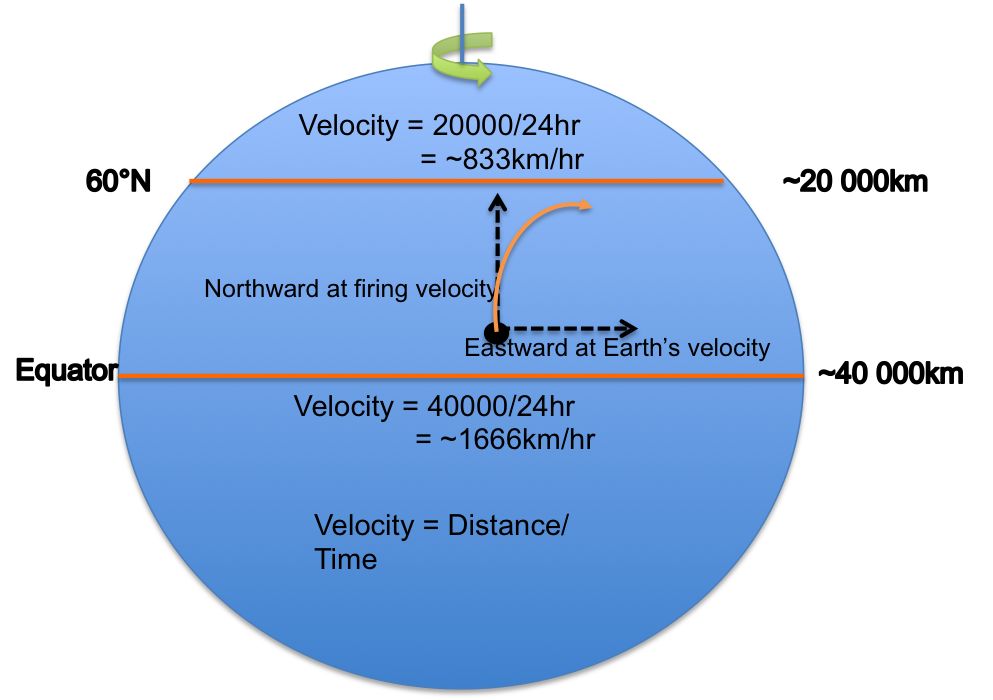
\includegraphics[scale=0.4]{figures/M3/coriolis_effect.png}
\par\end{center}
\begin{itemize}
\item The Coriolis effect is appreciated thinking of a missile fired northward
(or southward) from the equator to the poles. The deflection that
appears in the trajectory in relation to the Earth is due to the different
(linear) velocity of the Earth at different latitudes
\item It is a matter of "systems of reference" 
\end{itemize}
\end{frame}

\begin{frame}{Gaspard Gustave de Coriolis (1792-1843)}

\begin{columns}[t]


\column{7cm}

{\footnotesize{}We owe the understanding of this essential physical
principle to Gaspard Gustave de Coriolis. Born in France and trained
as an engineer, he began a career in teaching and research at age
24. Fascinated by problems related to rotating machinery, he was led
to derive the equations of motion in a rotating framework of reference.
The result of these studies was presented to the Academie des Sciences
in the summer of 1834. In 1838, Coriolis stopped teaching to become
director of studies at the Ecole Polytechnique, but his health declined
quickly and he died a few years later.}{\footnotesize\par}

{\footnotesize{}The world\textquoteright s largest experimental rotating
table, at LEGI (Laboratoire des Ecoulements Geophysiques et Industriels)
Grenoble, France, is named after him }


\column{6cm}
\begin{center}
\vspace{0cm}
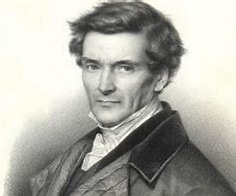
\includegraphics[width=3cm]{figures/M3/coriolis_pic.jpg}
\par\end{center}

\begin{center}
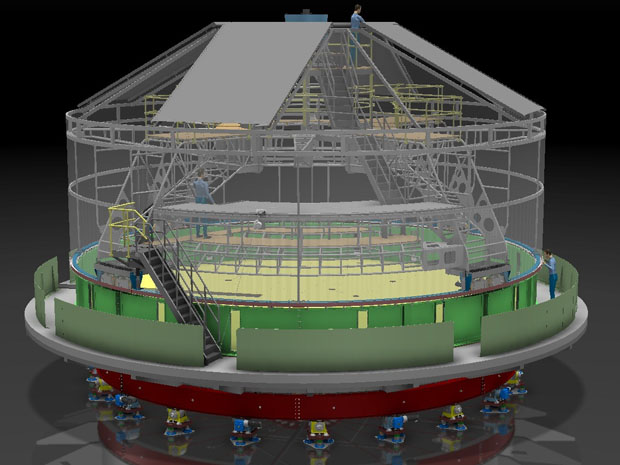
\includegraphics[width=6cm]{figures/M3/coriolis_platform.jpg}
\par\end{center}

\end{columns}

\end{frame}

\begin{frame}{Laboratory experiments in geophysical fluid dynamics}

\begin{columns}[c]


\column{6cm}
\begin{itemize}
\item {\small{}Most of the geophysical fluid dynamics processes are scalable,
which means that certain equilibria that are observed at planetary
scales can be reproduced in an appropriate laboratory setup}{\small\par}
\item {\small{}These experiments can be done using a rotating tank, to simulate
the rotation of the Earth}{\small\par}
\item {\small{}Check the experiments that can be done using a rotating apparatus:
\url{http://weathertank.mit.edu/links/projects}}{\small\par}
\end{itemize}

\column{6cm}

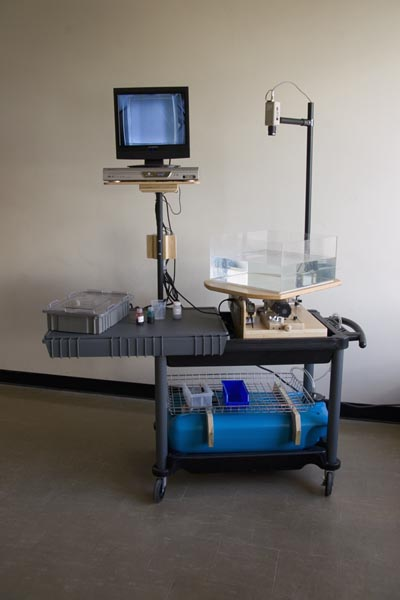
\includegraphics[scale=0.5]{figures/M1/Turntable_Cart}
\end{columns}

\end{frame}


\section{Forces due to rotation}
\begin{frame}{Forces due to rotation}

\begin{itemize}
\item These forces, \textbf{called apparent} forces, are generated by the
application of Newton's law in a rotating system
\begin{itemize}
\item \textbf{the centrifugal force }
\item \textbf{the Coriolis force}
\end{itemize}
\item The Earth rotation rate is called the\textbf{ angular velocity} (a
round angle \emph{in radians} divided by the rotation period \emph{in
s}). $\Omega=2\pi/\tau$ where $\tau$ is the length of the \href{https://en.wikipedia.org/wiki/Sidereal_time}{sidereal day}
(86164 s; the period of the Earth revolution around the sun divided
by the number of daily rotations). 
\[
\Omega=7.29\,10^{-5}\ s^{-1}
\]
(technically radians/s but radians have no units)
\end{itemize}
\end{frame}

\begin{frame}{The centrifugal force}

\begin{columns}[t]


\column{7cm}
\begin{itemize}
\item {\small{}The centrifugal force is the }\textbf{\small{}apparent outward
force acting on a mass when it rotates}{\small{}, like a ball at the
end of a string. This is the outward motion you feel in a car that
is turning (which is a non-inertial system). }{\small\par}
\item {\small{}The ball or the car have a constant linear velocity $V=\Omega r$
if seen from an external system of reference but the direction changes
over time, which means there is an apparent acceleration in the rotating
system ($r$ is the radius of rotation)}{\small\par}
\item {\small{}The centrifugal acceleration is compensated by a centripetal
acceleration. This is the real force!}{\small\par}
\end{itemize}

\column{7.5cm}
\begin{center}
\vspace{-1cm}
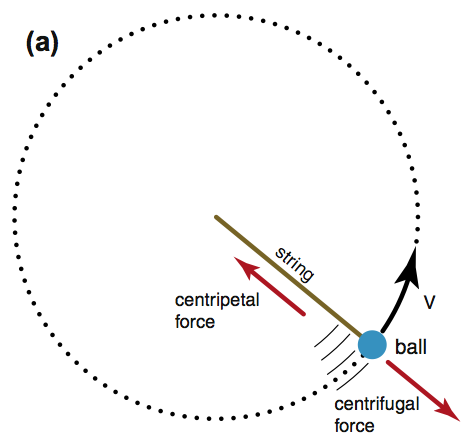
\includegraphics[width=4.5cm]{figures/M3/centrifugal.png}
\par\end{center}
\begin{itemize}
\item {\small{}In the string-ball system, it is the tension of the string
and in the rotating Earth it's gravity. The centrifugal acceleration
has the mathematical form $a_{cf}=\Omega^{2}r$. }\emph{\small{}Why
don't we feel the centrifugal acceleration? (wait a few slides)}{\small\par}
\end{itemize}
\end{columns}

\end{frame}

\begin{frame}{The Coriolis force}

\begin{columns}[t]


\column{7cm}
\begin{itemize}
\item {\footnotesize{}The Coriolis force }\emph{\footnotesize{}exists}{\footnotesize{}
for each object moving in a rotating system. }\textbf{\footnotesize{}It
is zero if it doesn't move.}{\footnotesize{} Although it is not a
real force in a fixed system of coordinates, it is real enough from
the point of view of anything moving in relation to the Earth. It
can be accurately computed and used to make predictions. }{\footnotesize\par}
\item {\footnotesize{}The Coriolis force }\textbf{\footnotesize{}changes
with latitude}{\footnotesize{}. It is 0 at the equator and maximum
at the poles}{\footnotesize\par}
\item {\scriptsize{}The Coriolis force is 3-dimensional: wind is deflected
also when the movement is vertical (but vertical velocities are small,
so deflection is small)}{\scriptsize\par}
\end{itemize}

\column{7.5cm}
\begin{center}
\vspace{-1cm}
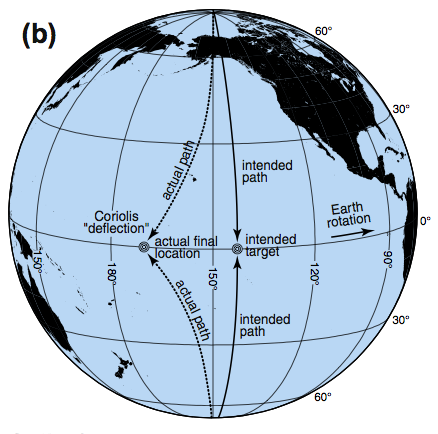
\includegraphics[width=4cm]{figures/M3/coriolis.png}
\par\end{center}
\begin{itemize}
\item \vspace{-0.7cm}
{\scriptsize{}On the Earth surface }\textbf{\scriptsize{}the Coriolis
force can be simplified through the Coriolis parameter}{\scriptsize{}
$f=2\Omega\sin\theta$ with $\theta$ the latitude (more later). The
acceleration acting on the fluid with velocity $U$ is $a_{c}=fU$}{\scriptsize\par}
\item {\scriptsize{}Given a certain latitude, the Coriolis parameter (and
the deflecting force) varies around it, increasing towards the pole
and decreasing towards the equator. It can be approximated as a linear
function of the latitudinal distance called the $\beta$-effect, where
$\beta$ is the derivative of $f$ along the N-S axis (more in next
modules) }{\scriptsize\par}
\end{itemize}
\end{columns}

\end{frame}


\section{Derivation of the apparent forces}
\begin{frame}{Transformation into rotating coordinates}

\begin{columns}[t]


\column{7.5cm}

{\footnotesize{}A fixed point in a system of coordinates is identified
with a position vector $\mathbf{r}\equiv\left(x,y,z\right)$. If the
same system of coordinates rotates in another inertial system of coordinates,
what are the new coordinates?}{\footnotesize\par}
\begin{itemize}
\item {\scriptsize{}It can be demonstrated that the time rate of change
of a vector $\mathbf{A}$ in a rotating system is seen in the inertial
system as
\[
\left(\frac{D\mathbf{A}}{Dt}\right)_{in}=\left(\frac{D\mathbf{A}}{Dt}\right)_{rot}+\boldsymbol{\Omega}\times\mathbf{A}
\]
where $\boldsymbol{\Omega}$ is the angular velocity vector of the
rotating frame (in the inertial system). }\emph{\scriptsize{}Remember
that we need a vector to identify the plane of rotation; the angular
velocity is the magnitude}{\scriptsize\par}
\item {\scriptsize{}If we use the vector representing the fixed point in
the rotating frame, we get the linear velocity of the point in the
inertial frame}{\scriptsize\par}
\end{itemize}

\column{6cm}

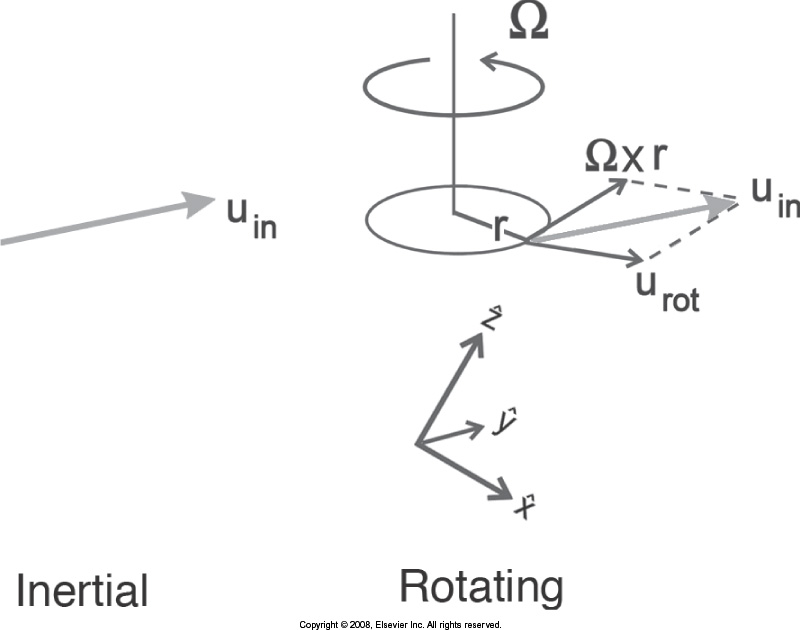
\includegraphics[width=5cm]{figures/M3/f06-09-P558691}

{\scriptsize{}
\[
\left(\frac{D\mathbf{r}}{Dt}\right)_{in}=\mathbf{u}_{in}=0+\boldsymbol{\Omega}\times\mathbf{r}
\]
If the point was moving with velocity $\mathbf{u}_{rot}$ as in the
example picture above, then we would get
\[
\mathbf{u}_{in}=\mathbf{u}_{rot}+\boldsymbol{\Omega}\times\mathbf{r}
\]
}{\scriptsize\par}
\end{columns}

\end{frame}

\begin{frame}{Acceleration in a rotating frame}

\begin{itemize}
\item What is the acceleration of the fluid in the rotating framework?
\item We compute the derivative of the velocity in the inertial system using
the expression $\mathbf{u}_{in}=\mathbf{u}_{rot}+\boldsymbol{\Omega}\times\mathbf{r}$,
remembering that $\Omega$ is constant,
\begin{align}
\left(\frac{D\mathbf{u}_{in}}{Dt}\right)_{in} & =\left(\frac{D\left(\mathbf{u}_{rot}+\boldsymbol{\Omega}\times\mathbf{r}\right)}{Dt}\right)_{rot}+\boldsymbol{\Omega}\times\left(\mathbf{u}_{rot}+\boldsymbol{\Omega}\times\mathbf{r}\right)=\nonumber \\
 & =\left(\frac{D\mathbf{u}_{rot}}{Dt}\right)_{rot}+\boldsymbol{\Omega}\times\left(\frac{D\mathbf{r}}{Dt}\right)_{rot}+\boldsymbol{\Omega}\times\mathbf{u}_{rot}+\boldsymbol{\Omega}\times\boldsymbol{\Omega}\times\mathbf{r}=\nonumber \\
 & =\left(\frac{D\mathbf{u}_{rot}}{Dt}\right)_{rot}+2\boldsymbol{\Omega}\times\mathbf{u}_{rot}+\boldsymbol{\Omega}\times\boldsymbol{\Omega}\times\mathbf{r}\label{eq:inertial_acceleration}
\end{align}
where we have recognized that 
\[
\left(\frac{D\mathbf{r}}{Dt}\right)_{rot}=\mathbf{u}_{rot}
\]
\end{itemize}
\end{frame}

\begin{frame}{The equations of motions in a rotating system}

\begin{itemize}
\item We now have everything to transform the Navier-Stokes equations we
derived for an inertial system: 
\[
\frac{D\mathbf{u}_{in}}{Dt}=-\frac{\nabla p}{\rho}-g\,\mathbf{\hat{k}}+\boldsymbol{\mathcal{F}}
\]
 into the ones valid for a rotating frame. Notice that all the scalar
fields are not affected by rotation: density remains density and the
same for pressure
\item We only need to substitute the definition of inertial acceleration
obtained in eq. (\ref{eq:inertial_acceleration}) in the rotating
framework. Now the unit vectors are the ones of the rotating system,
we rename $\mathbf{u}_{rot}$ simply $\mathbf{u}$,and we use the
gravity and friction forces observed in the rotating system. By developing
all terms, we obtain two new \emph{apparent} accelerations:
\begin{equation}
\boxed{\frac{D\mathbf{u}}{Dt}=-\frac{\nabla p}{\rho}-g\,\mathbf{\hat{k}}\underbrace{-2\boldsymbol{\Omega}\times\mathbf{u}}_{\textrm{Coriolis}}\underbrace{-\boldsymbol{\Omega}\times\boldsymbol{\Omega}\times\mathbf{r}}_{\textrm{Centrifugal}}+\boldsymbol{\mathcal{F}}}\label{eq:NS-rotating}
\end{equation}
\end{itemize}
\end{frame}

\begin{frame}{The Coriolis acceleration}

\begin{columns}[t]


\column{5cm}

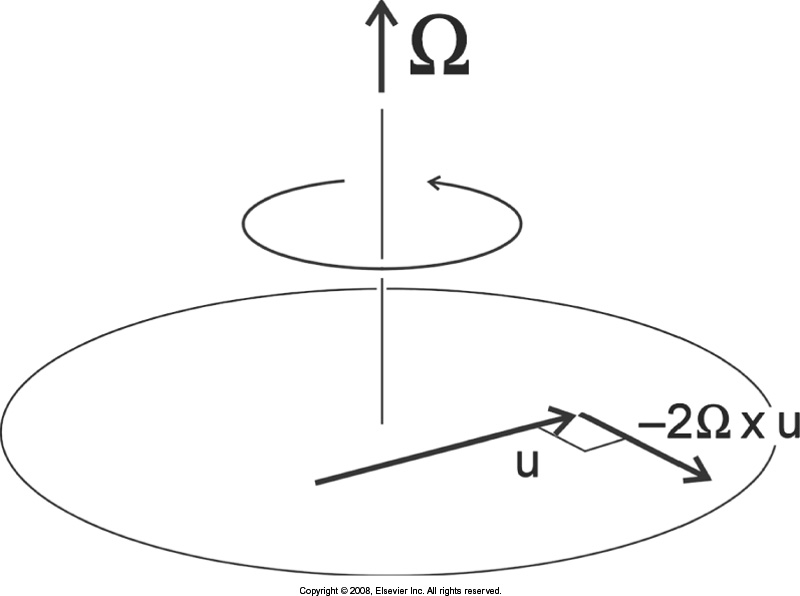
\includegraphics[width=4.5cm]{figures/M3/f06-10-P558691}

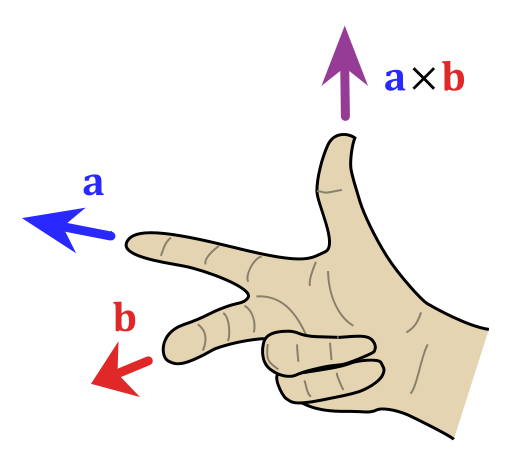
\includegraphics[width=4.5cm]{figures/M3/Right_hand_rule_cross_product}

\column{6cm}
\begin{itemize}
\item It is an apparent force, \emph{generated} in the rotating system by
the balance of forces in the inertial system
\item Apply the right hand rule to check the direction or compute the cross-product
with the determinant
\end{itemize}
\end{columns}

\end{frame}


\section{Inertial oscillations}
\begin{frame}{A natural motion of the ocean: inertial oscillations}

\begin{columns}[t]


\column{7cm}

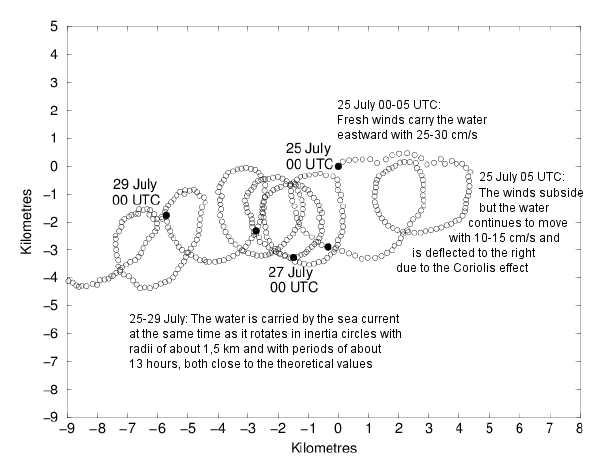
\includegraphics[width=6cm]{figures/M3/inertia_circle}
\begin{itemize}
\item {\footnotesize{}It is not unusual to observe circular motion in oceanic
floats or sea-ice floes. The trajectory follows the so-called inertial
cycles with a period depending on the local value of $\Omega$. }\textbf{\footnotesize{}This
value is called the Coriolis parameter}{\footnotesize{} $f=2\Omega\sin\theta$
(see next slide for a full derivation)}{\footnotesize\par}
\end{itemize}

\column{7cm}
\begin{itemize}
\item {\footnotesize{}If a fluid parcel has a velocity and there are no
other forces in eq. (\ref{eq:NS-rotating}), then the particle would
accelerate with
\[
\frac{D\mathbf{u}}{Dt}=-2\boldsymbol{\Omega}\times\mathbf{u}
\]
The full derivation of the resulting circular motion in the rotating
framework is shown in the M\&P textbook Lab V at pag. 97. }{\footnotesize\par}
\item {\footnotesize{}The acceleration just deviates the flow to the right
or left depending on the sign of $\boldsymbol{\Omega}$, but it }\emph{\footnotesize{}does
no work}{\footnotesize{} because it is orthogonal to the motion. Try
to compute $\left(\boldsymbol{\Omega}\times\mathbf{u}\right)\cdot\mathbf{u}$,
and you'll see that it is zero, which means no energy dissipation
(\url{http://www.cleonis.nl/physics/phys256/inertial_oscillations.php})}{\footnotesize\par}
\end{itemize}
\end{columns}

\end{frame}


\section{The Coriolis parameter (derivation)}
\begin{frame}{The Coriolis parameter (on the sphere)}

\begin{columns}[c]


\column{3.5cm}

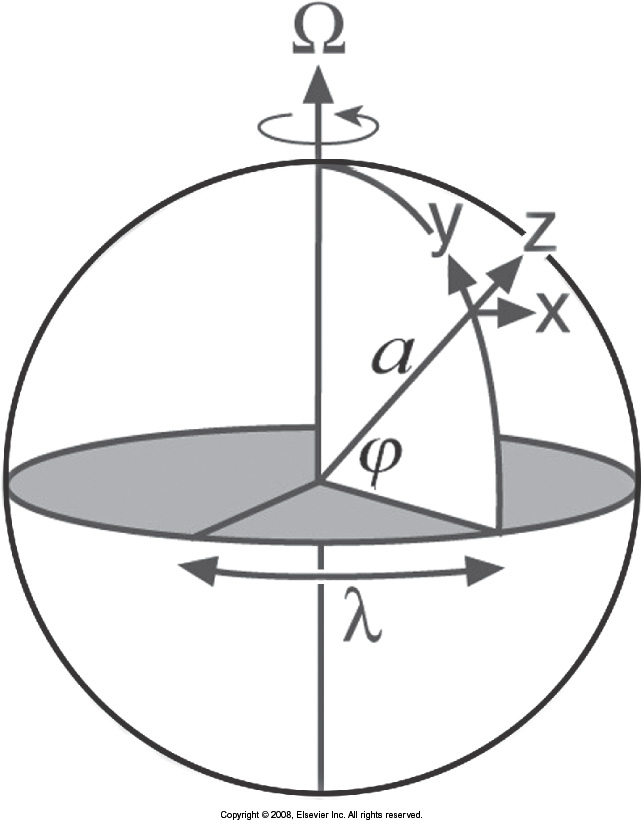
\includegraphics[width=3.5cm]{figures/M3/f06-19-P558691}

\column{10.5cm}
\begin{itemize}
\item {\footnotesize{}The equations of motions have to describe fluids on
the sphere and not on a rotating disc. It is therefore convenient
to use a system of coordinates that follows the curvature: }\emph{\footnotesize{}terrestrial
coordinates (the axes x-y-z in the figure, which depend on $\lambda$
and $\theta$)}{\footnotesize\par}
\item {\footnotesize{}$\boldsymbol{\Omega}$ has only 2 components in this
system, N-S and the vertical, $\left(0,\Omega\cos\theta,\Omega\sin\theta\right)$
and the Coriolis acceleration becomes (using $\mathbf{u}\equiv\left(u,v,w\right)$)
\[
-2\boldsymbol{\Omega}\times\mathbf{u}=-2\Omega\left(w\cos\theta-v\sin\theta\right)\hat{\mathbf{i}}-2\Omega u\sin\theta\hat{\mathbf{j}}-2\Omega u\cos\theta\hat{\mathbf{k}}
\]
}{\footnotesize\par}
\item \emph{\footnotesize{}Coriolis has a vertical component}{\footnotesize{}
in this system of coordinates. It is however very small if compared
to gravity. Also, the vertical velocities of geophysical fluids are
much smaller than the horizontal. We thus make two reasonable simplifications
and write 
\[
-2\boldsymbol{\Omega}\times\mathbf{u}\approx2\Omega v\sin\theta\hat{\mathbf{i}}-2\Omega u\sin\theta\hat{\mathbf{j}}+0\hat{\mathbf{k}}=-f\hat{\mathbf{k}}\times\mathbf{u}
\]
where we have defined }\textbf{\footnotesize{}the Coriolis parameter}{\footnotesize{}
$f=2\Omega\sin\theta$}{\footnotesize\par}
\end{itemize}
\end{columns}

\end{frame}


\section{The centrifugal acceleration (derivation)}
\begin{frame}{The Centrifugal acceleration on the sphere}

\begin{columns}[t]


\column{7cm}

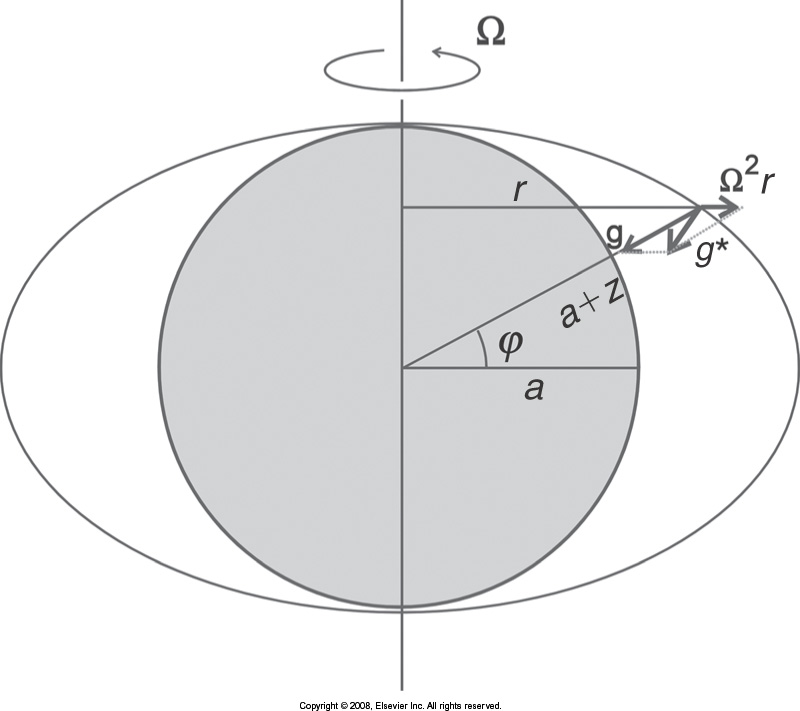
\includegraphics[width=5cm]{figures/M3/f06-18-P558691}

{\footnotesize{}Gravity and the centrifugal force acted over geological
time and adjusted the surface of the Earth to an equipotential surface,
close to an ellipsoid. The gravity we measure, $g^{*}$ in the figure,
is the combination of both forces (this is exaggerated: the bulge
is just 21 km)}{\footnotesize\par}

\column{7.5cm}
\begin{itemize}
\item {\footnotesize{}$\boldsymbol{-\Omega}\times\boldsymbol{\Omega}\times\mathbf{r}$
is directed radially outwards with magnitude $-\Omega^{2}r$ and $r$
is the distance from the axis of the Earth. We write everything in
terms of the Earth radius $a=6371$ km: $r=\left(a+z\right)\cos\theta\approxeq a\cos\theta$
because we assume that the ocean and the atmosphere are ``shallow''.}{\footnotesize\par}
\item {\footnotesize{}On the ellipsoid, }\textbf{\footnotesize{}this apparent
acceleration is combined with gravity to give the modified or resultant
gravity}{\footnotesize{} (which is the one measured on the Earth surface
along the direction of plumb lines). It is expressed in terms of a
}\emph{\footnotesize{}gravitational potential, the gradient of which
is equal to the acceleration }{\footnotesize{}
\[
\phi(z)=gz-\frac{\Omega^{2}a^{2}\cos^{2}\theta}{2}
\]
}{\footnotesize\par}
\end{itemize}
\end{columns}

\end{frame}


\section{The Navier-Stokes equations for GFD}
\begin{frame}{The Navier-Stokes equations for GFD}

\begin{itemize}
\item We now add the effects of rotation to the momentum balance derived
in the previous section. The N-S equations in vector form are written
combining all terms
\[
\boxed{\underbrace{\ \frac{D\mathbf{u}}{Dt}\ }_{\textrm{Total acceleration}}=\underbrace{-\frac{\nabla p}{\rho}}_{\textrm{Pressure gradient}}\underbrace{-f\mathbf{\hat{k}}\times\mathbf{u}}_{\textrm{Coriolis}}\underbrace{-\nabla\phi}_{\textrm{Geopotential}}\underbrace{+\boldsymbol{\mathcal{F}}}_{\textrm{Friction}}}
\]
\item The components on the terrestrial coordinate system, also applying
the hydrostatic equilibrium, are
\begin{align*}
\frac{Du}{Dt} & =-\frac{1}{\rho}\frac{\partial p}{\partial x} & +fv & +F_{x}\\
\frac{Dv}{Dt} & =-\frac{1}{\rho}\frac{\partial p}{\partial y} & -fu & +F_{y}\\
\frac{1}{\rho}\frac{\partial p}{\partial z} & = & -g
\end{align*}
\end{itemize}
\end{frame}


\end{document}
